\documentclass[journal, twocolumn]{IEEEtran}
\usepackage[acronym]{glossaries}
\usepackage{lineno,hyperref}
\usepackage[margins]{trackchanges}
\usepackage{cite}
%\usepackage{xcolor}
%\usepackage{amsmath,amssymb,amsfonts}
%\usepackage{algorithmic}
\usepackage[pdftex]{graphicx}
\DeclareGraphicsExtensions{.pdf,.jpeg,.png}
% \usepackage{subfigure}
% \usepackage{multirow}
% \usepackage{array}
% \usepackage{stfloats}
% \usepackage{textcomp}
% \usepackage{tikz}

% Include this file to add \mir{} \mar{} comments.

\usepackage[textsize=small,backgroundcolor=white]{todonotes}
\newcounter{Exe}
\newcommand{\mar}[1]{\refstepcounter{Exe} \textcolor{red}{\todo[inline]{\textbf{Major revision \#\arabic{Exe}}: #1}}}
\newcommand{\mir}[1]{\refstepcounter{Exe} \textcolor{blue}{\todo[inline]{\textbf{Minor revision \#\arabic{Exe}}: #1}}}

\newcommand{\rev}[1]{\textcolor{blue}{\textbf{Revise:}}\textcolor{red}{#1}}
    % remove this if there is no comments 
\newcommand{\maxwell}
{
\begin{align}
\nabla\times {\mathbf{E}}&=-\frac{\partial {\mathbf{B}}}{\partial t}  \\
\nabla\times {\mathbf{H}}&={\mathbf{J}}+\frac{\partial {\mathbf{D}}}{\partial t}  \\
\nabla\cdot {\mathbf{B}}&=0  \\
\nabla\cdot {\mathbf{D}}&=\rho 
\label{eq:maxwell}
\end{align}
}


\newcommand{\maxwella}
{\begin{align}
{\mathbf{B}}&=\mu {\mathbf{H}}  \\
{\mathbf{D}}&=\varepsilon {\mathbf{E}}  \\
{\mathbf{J}}&=\sigma {\mathbf{E}} 
\label{eq:maxwella}
\end{align}
}


\newcommand{\ect}
{
\begin{equation}
   \nabla \cdot\left(\varepsilon \nabla \varphi \right)=0
\label{eq:ect}
\end{equation}
}

\newcommand{\ecrt}
{
\begin{equation}
  \nabla \cdot\left[(\sigma +j\omega \varepsilon )\nabla \varphi \right]=0
\label{eq:ecrt}
\end{equation}}

\newcommand{\ectb}
{
\begin{equation}
\left\{
\begin{array}{rl}
    \varphi_{\Gamma_e}=&V_e\\
    \varphi_{\Gamma_m}=&0\\
    \varphi_{\Gamma_{s}}=&0\\
\end{array}
\right.  
\label{eq:ectb}
\end{equation}
}


\newcommand{\capacitance}
{
\begin{equation}
  C=\frac{Q}{V_e}=-\frac{1}{V_e}\int_{\Omega_m}\varepsilon(x,y,z)\nabla\varphi(x,y,z) d\Omega
\label{eq:capacitance}  
\end{equation}
}

\newcommand{\emt}
{
\begin{equation}
  \nabla\times \left[\left(\nabla \times \frac{\mathbf{B}}{\mu}\right)/\sigma\right]=-j\omega \mathbf{B}  
  \label{eq:emt}
\end{equation}
}

\newcommand{\emta}
{
  \begin{equation}
  \nabla^2\mathbf{A}+j\omega\mu\sigma \mathbf{A}=\mu \mathbf{J}
  \label{eq:emta}
\end{equation}
}


\newcommand{\deltaz}
{
  \begin{align}
    \Delta Z &= \frac{1}{I^2}\int_{\Omega}j\omega(\mu_x-\mu_0)\mathbf{H}_x\cdot\mathbf{H}_0 \nonumber\\
    &-(\sigma_x-\sigma_0+j\omega\varepsilon_x-j\omega\varepsilon_0)\mathbf{E}_x\cdot\mathbf{E}_0 d\Omega
    \label{eq:deltaz}
  \end{align}
}


\newcommand{\snr}
{
  \begin{equation}
    \mathbf{SNR} = -20\lg\left[\frac{1}{\mu}\sqrt{\frac{1}{n}\sum\limits_{i=1}^{n}(x_i-\mu)^{2}}\right]
    \label{eq:snr}
  \end{equation}
}


\newcommand{\snrd}
{
  \begin{equation}
    \mathbf{SNR_\Delta} = -20\lg\left[\frac{1}{|\mu_h-\mu_l|}\sqrt{\frac{1}{n}\sum\limits_{i=1}^{n}(x_i-\mu_h)^{2}}\right]    \label{eq:snrd}
  \end{equation}
}

\newcommand{\corrcoe}
{
  \begin{equation}
    r=\frac{\sum_{i=1}^{N}\left(\hat{\mathbf{g}}_{i}-\overline{\hat{\mathbf{g}}}\right)\left(\mathbf{g}_{i}-\overline{\mathbf{g}}\right)}{\sqrt{\sum_{i=1}^{N}\left(\hat{\mathbf{g}}_{i}-\overline{\hat{\mathbf{g}}}\right)^{2} \sum_{i=1}^{N}\left(\mathbf{g}_{i}-\overline{\mathbf{g}}\right)^{2}}}
    \label{eq:corrcoe}
  \end{equation}
}

\newcommand{\rmse}{
  \begin{equation}
    \mathbf{RMSE} = \sqrt{\frac{1}{N}\sum_{i=1}^{N}(\hat{\delta}_{i} - \delta_{i})^2}
    \label{eq:rmse}
  \end{equation}
}

\newcommand{\emap}
{
  \begin{equation}\label{eq:normc}
    \delta_h^p = \frac{C_{e}-C_{l}}{C_{h}-C_{l}}
    \end{equation}
}

\newcommand{\emas}
{
  \begin{equation}\label{eq:emas}
    \delta_h^s = \frac{C_{h}}{C_{e}}\frac{(C_{e}-C_{l})}{(C_{h}-C_{l})}=\left(\frac{C_h}{C_e}\right)\delta_h^p
  \end{equation}
}

\newcommand{\emamg}
{
  \begin{equation}\label{eq:emamg}
    \delta_{h}^{MG}
    =\frac{(C_{h}+2C_{l})}{(C_{e}+2C_{l})}\frac{(C_{e}-C_{l})}{(C_{h}-C_{l})}
    =\left(\frac{C_{h}+2C_{l}}{C_{e}+2C_{l}}\right) \delta_h^p
    \end{equation}
}

\newcommand{\emabo}{
  \begin{equation}\label{eq:emabo}
  \delta_h^{Bo}=
  \frac{(C_h+2C_e)}{3C_e}\frac{(C_{e}-C_{l})}{(C_{h}-C_{l})}
  =\left(\frac{2C_{e}+C_{h}}{3C_{e}}\right)\delta_h^p
\end{equation}
}

\newcommand{\emabr}{
  \begin{equation}\label{eq:emabr}
  \delta_h^{Br}= \frac{C_{e}+C_{h}}{2C_{e}}\frac{(C_{e}-C_{l})}{(C_{h}-C_{l})}
  =\left(\frac{C_{e}+C_{h}}{2C_{e}}\right)\delta_h^p
\end{equation}
}

\newcommand{\emft}{
  \begin{equation} \label{eq:emft}
    \nabla \cdot \sigma \nabla \varphi = \nabla \cdot \sigma (\vec {v} \times \vec {B}), 
\end{equation}
}


\newcommand{\emftb}{
  \begin{align*} 
    \frac {\partial \varphi}{\partial \hat {n}}=&0, \quad \vec {r} \in \partial \Omega, 
    \\ 
    \vec {v}=&0, \quad \vec {r} \in \partial \Omega _{\mathrm{wall}}, 
    \\ 
    \vec {B}=&0, \quad \vec {r} \in \partial \Omega _{\mathrm{ends}}, 
  \end{align*}  
}





\hyphenation{op-tical net-works semi-conduc-tor}


\begin{document}

\title{Bare Demo of IEEEtran.cls\\ for IEEE Journals}


\author{
  Ziqiang Cui,~\IEEEmembership{Member,~IEEE,}
  Andy~Lau, 
  and~Huaxiang~Wang,~\IEEEmembership{Senior~Member,~IEEE}% <-this % stops a space
\thanks{Dr. Ziqiang Cui was with the School of
of Electrical and Information Engineering, Tianjin University, Tianjin 300072, China.
Correspondance e-mail: cuiziqiang@tju.edu.cn.}% <-this % stops a space
\thanks{This research is financially supported by NSFC, Nos. 61671319 and 61627803.}% <-this % stops a space
\thanks{Manuscript updated \today and submitted Feb 28, 2020.}}

\maketitle

\begin{abstract}
The abstract goes here.
\end{abstract}

\begin{IEEEkeywords}
IEEE, IEEEtran, journal, \LaTeX, paper, template.
\end{IEEEkeywords}


\annote{Text}{Blablabla...abcdef}



\IEEEpeerreviewmaketitle



% Sections

%!TEX root = ../article.tex

% Introduction
\section{Introduction}
\label{sec:introduction}


\IEEEPARstart{T}{his} is a well organized \LaTeX ~template for the IEEE papers that can be used by  the graduate students to prepare the IEEE conference and journal papers.



\subsection{Titles}

One can modify the author list, institution, address, correspondence email and title of paper in the file \verb+article.tex+.



\subsection{Math formula}

Some frequently used formulas can be found in the file \verb+math.tex+.
To refer a formula, use the corresponding command.
For example, we can add the Maxwell's equations as \verb+\maxwell+, and produce:

\maxwell

More formated equations are summerized  in the appendix.



\subsection{Bibliography}

We can use the Jabref software to manage the bibliography.
The file \verb+bib.bib+ can be used as a common library to add references to the manuscript.

\begin{itemize}
  \item Add BibTeX Entry: On the website (https://ieeexplore.ieee.org), click the button ``Download citations'' and choose output format ``BibTeX''. Copy the text and paste it into the file \verb+bib.bib+ by using Jabref (New BibTeX entry, BibTeX source).
  \item Merge Multiple Bibliography files: In Jabref, Import into current library, Deselect all duplicates, Save.
  \item Insert Citations: This is an example in how to cite a bibliography entry \cite{cao2018, cui2019}.
\end{itemize}

\subsection{IEEE LaTeX Analyzer}
The IEEE LaTeX Analyzer is an online service, built to assist authors with validating their LaTeX article packages. The tool provides detailed results for uploaded LaTeX packages, along with a resource for correcting any LaTeX issues, if needed. The IEEE LaTeX Analyzer can be used at any time, with one ideal use being prior to peer review article submission. Validating LaTeX article packages prior to submission helps to ensure the fastest possible speed to publication.
The website is:
\verb+http://latexqc.ieee.org/+

%!TEX root = ../article.tex

% Entry point for sections:
%
% This file specifies the sections and  its respective order in which they must
% be included.

% Article Sections
\section{Methods}
\label{sec:methods}

\subsection{How to improve the academic English writing}

The easiest way is to \ldots

\begin{itemize}
  \item Find 10 or more relevant papers that wrote by the native speakers, read and memorize the classic sentences.
  \item Learn how to describe and discuss the results, figures and tables; conclude the work and demonstrate the significance.
  \item Keep in mind that \textbf{NO PLAGIARISM} is allowed.
  \item One can avoid plagiarism by word-by-word rephrasing the sentences.
\end{itemize}


\subsection{Figures \& Tables}

Use of figures and tables to illustrate the results should be firstly considered.

\begin{figure}[h]
  \centering
  \includegraphics[width=0.6\columnwidth]{../figure_examples/circuit/simple.pdf}
  \caption{Circuit sample.}
  \label{fig:circuit_simple}
\end{figure}



\renewcommand\arraystretch{1.8}
\begin{table}
\caption{Summery of effective medium approximation formulas.}\label{tab:formula}
  \centering
  \begin{tabular}{lll}
  \hline
Relation & Formula &  Correction factor \\
\hline
Parallel/Linear &  $\delta_h^p = \frac{\varepsilon_{e}-\varepsilon_{l}}{\varepsilon_{h}-\varepsilon_{l}}$
       &   1 \\
Series & $\delta_h^s= \frac{\varepsilon_{h}}{\varepsilon_{e}}\frac{(\varepsilon_{e}-\varepsilon_{l})}{(\varepsilon_{h}-\varepsilon_{l})}$
& $\left(\frac{\varepsilon_h}{\varepsilon_e}\right)$\\
 Maxwell-Garnett &
$\delta_{h}^M
=\frac{(\varepsilon_{h}+2\varepsilon_{l})}{(\varepsilon_{e}+2\varepsilon_{l})}\frac{(\varepsilon_{e}-\varepsilon_{l})}{(\varepsilon_{h}-\varepsilon_{l})}
$&$\left(\frac{\varepsilon_{h}+2\varepsilon_{l}}{\varepsilon_{e}+2\varepsilon_{l}}\right)$\\
Bruggeman &  $\delta_h^{Br}= \frac{\varepsilon_{e}+\varepsilon_{h}}{2\varepsilon_{e}}\frac{(\varepsilon_{e}-\varepsilon_{l})}{(\varepsilon_{h}-\varepsilon_{l})}$
& $\left(\frac{\varepsilon_{e}+\varepsilon_{h}}{2\varepsilon_{e}}\right)$\\
B\"{o}ttcher &  $\delta_h^{Bo}=
  \frac{(\varepsilon_h+2\varepsilon_e)}{3\varepsilon_e}\frac{(\varepsilon_{e}-\varepsilon_{l})}{(\varepsilon_{h}-\varepsilon_{l})}$
&$ \left(\frac{2\varepsilon_{e}+\varepsilon_{h}}{3\varepsilon_{e}}\right)$ \\ \hline
  \end{tabular}
\end{table}
\renewcommand\arraystretch{1}


\subsection{Tips}

\emph{i.e.}

%!TEX root = ../article.tex

% Entry point for sections:
%
% This file specifies the sections and  its respective order in which they must
% be included.

% Article Sections
\section{Results and Discussions}
\label{sec:results} 


%!TEX root = ../dissertation.tex

% Conclusion
\section{Conclusion}
\label{sec:conclusion}


%
\appendices
\section{Common Equations List}

The label for  equation \verb+\xxx+ is \verb+\label{eq:xxx}+.

\begin{itemize}
  \item \verb+\maxwell+ : 
  \maxwell
  \item \verb+\maxwella+ 
  \maxwella
  \item The electrostatic field equation: \verb+\ect+
   \ect
  \item The electric field equation considering applied frequency: \verb+\ecrt+
  \ecrt
  \item Boundary conditions for ECT sensor: \verb+\ectb+
  \ectb
  \item The equation for calculating the inter-electrode capacitances: \verb+\capacitance+
  \capacitance
  \item The dominant equation for EMT: \verb+\emt+
  \emt,
  and, \verb+\emta+
  \emta.
  \item \verb+\deltaz+
  \deltaz
  \item The signal-to-noise ratio (SNR) is defined as: \verb+\snr+
  \snr
  \item This signal-to-noise ratio is defined with respect to the difference between the high and low calibrations: \verb+\snrd+
  \snrd
  \item The correlation coefficient is employed for quantitatively evaluating the image quality: \verb+\corrcoe+
  \corrcoe
  \item Root mean square error: \verb+\rmse+
  \rmse
  \item A simple parallel EMA model: \verb+\emap+
  \emap
  \item The series model: \verb+\emas+
  \emas
  \item The Maxwell-Garnet model: \verb+\emamg+
  \emamg
  \item B\"{o}ttcher model: \verb+\emabo+
  \emabo
  \item Bruggeman model: \verb+\emabr+
  \emabr
  % \item \verb++

  % \item \verb++

  % \item \verb++

  % \item \verb++

  % \item \verb++

  % \item \verb++

  % \item \verb++

  % \item \verb++


\end{itemize}
 To add more \dots

\section*{Acknowledgment}

The authors would like to thank the financial supports from NSFC (Nos. 61671319 and 61627803).

\ifCLASSOPTIONcaptionsoff
  \newpage
\fi

% Bibliography
\bibliographystyle{IEEEtran}
% Bibliography file
\bibliography{../ieee-latex-template-v2/zotero}


% % biography section
%
% If you have an EPS/PDF photo (graphicx package needed) extra braces are
% needed around the contents of the optional argument to biography to prevent
% the LaTeX parser from getting confused when it sees the complicated
% \includegraphics command within an optional argument. (You could create
% your own custom macro containing the \includegraphics command to make things
% simpler here.)
%
% or if you just want to reserve a space for a photo:

%\begin{IEEEbiography}[{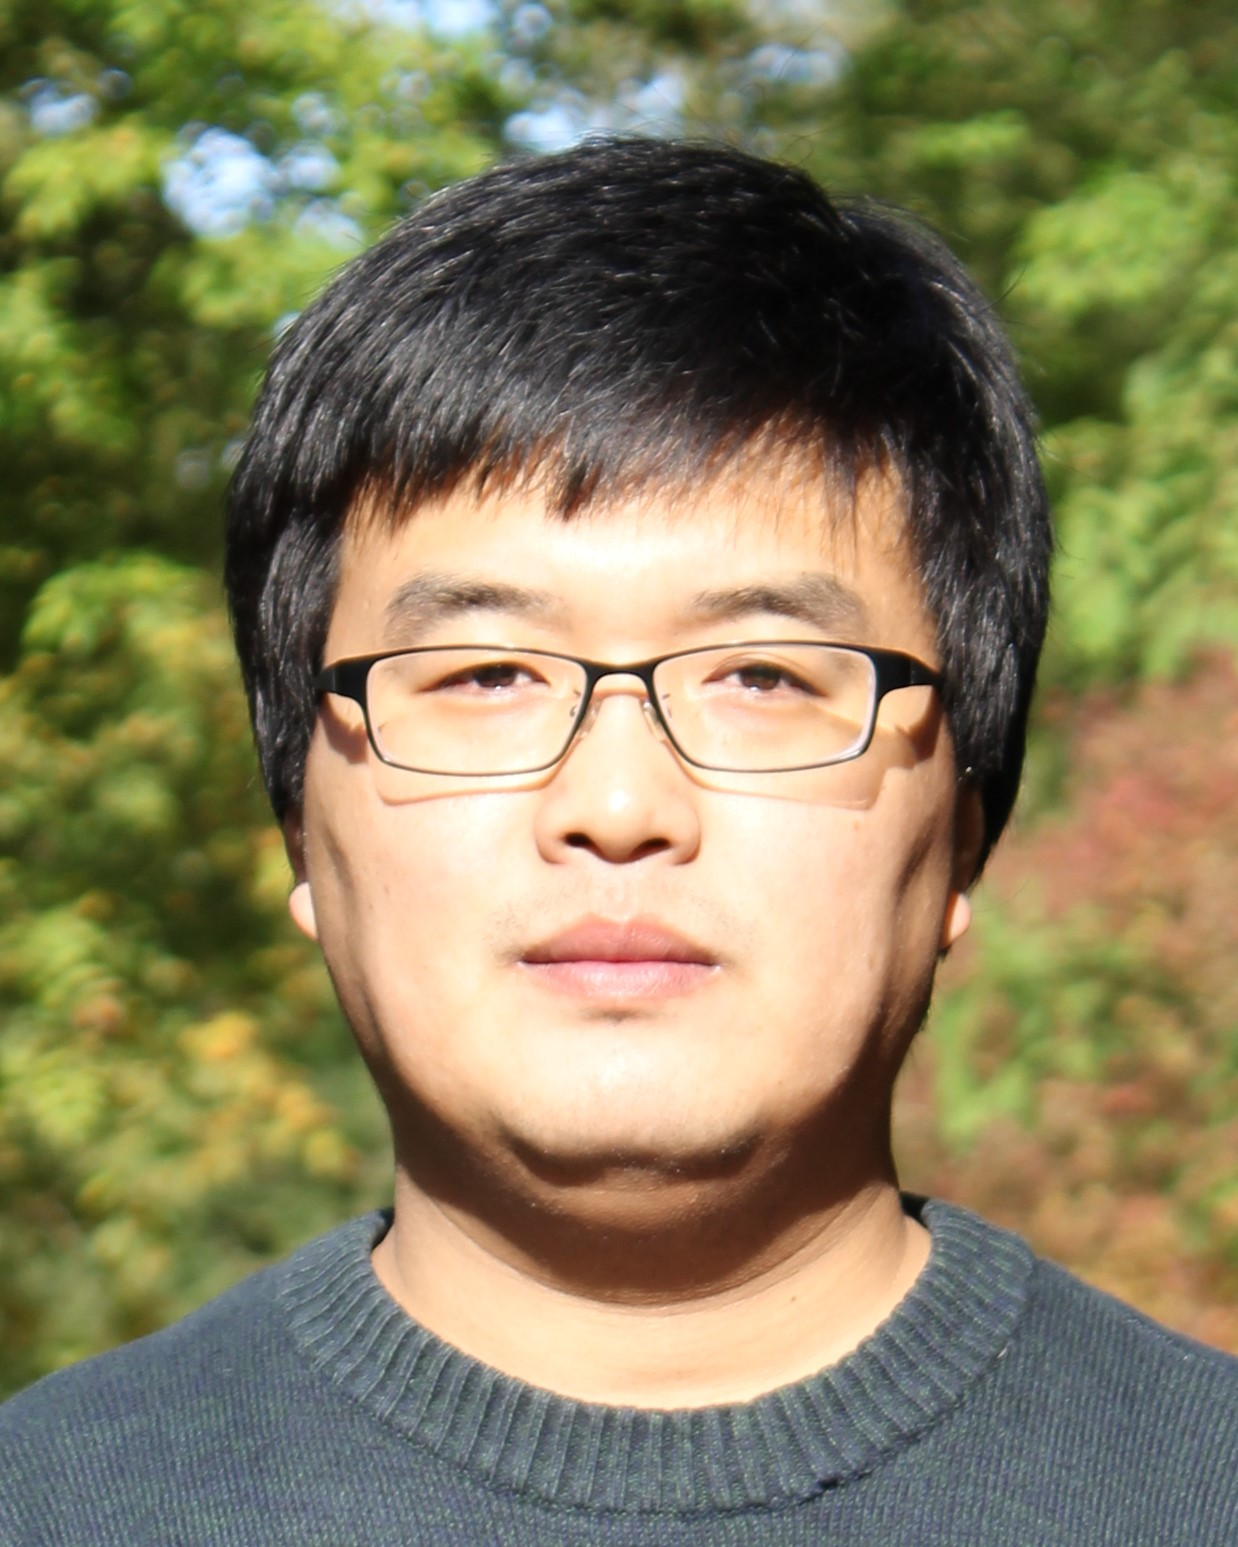
\includegraphics[width=1in,height=1.25in,clip,keepaspectratio]{figures/cui.jpg}}]{Ziqiang Cui}
%(M'13) received the M.Sc. and Ph.D. degrees from Tianjin University, China, in 2007 and 2009, respectively. He is currently an Associate Professor with the School of Electrical and Information Engineering, Tianjin University. His current research interests include electrical tomography instrumentation, signal processing, sensor design, and multi-phase flow measurement.
%\end{IEEEbiography}


\begin{IEEEbiography}[{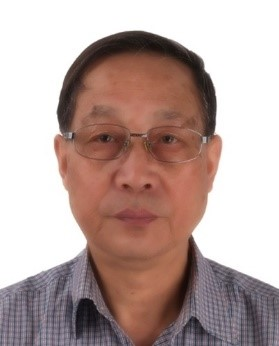
\includegraphics[width=1in,height=1.25in,clip,keepaspectratio]{figures/wang.jpg}}]{Huaxiang Wang}
(SM'06) received the degree from Tianjin University, China. He is currently a Professor with the School of Electrical and Information Engineering, Tianjin University.  His major research interests include sensing techniques and information processing, process parameter detection and control systems, and intelligent instrumentations.
\end{IEEEbiography}

% You can push biographies down or up by placing
% a \vfill before or after them. The appropriate
% use of \vfill depends on what kind of text is
% on the last page and whether or not the columns
% are being equalized.

\vfill

% Can be used to pull up biographies so that the bottom of the last one
% is flush with the other column.
%\enlargethispage{-5in}



% that's all folks 
\end{document}